\documentclass{sig-alternate-hotpets15}
\usepackage{color}
\usepackage[hyphens]{url}
\usepackage{longtable}
\usepackage{graphicx}
\usepackage{enumitem}
\usepackage{pdfpages}

\def\etal{{\it et al.~}}
\newenvironment{packed_enum}{
\begin{enumerate}
  \setlength{\itemsep}{1pt}
  \setlength{\parskip}{0pt}
  \setlength{\parsep}{0pt}
}{\end{enumerate}}
\newenvironment{packed_item}{
\begin{itemize}
  \setlength{\itemsep}{1pt}
  \setlength{\parskip}{0pt}
  \setlength{\parsep}{0pt}
}{\end{itemize}}

\begin{document}
\title{Risk Perceptions for Wearable Devices}
\numberofauthors{1}
\author{
 \alignauthor Linda N. Lee\textsuperscript{1}, Serge Egelman\textsuperscript{1,3}, Joong Hwa Lee\textsuperscript{2}, David Wagner\textsuperscript{1}\\
   \vspace{0.5em}
   \affaddr{\textsuperscript{1}University of California, Berkeley, \{lnl,egelman,daw\}@cs.berkeley.edu}, \textsuperscript{2}dlwndghk94@berkeley.edu\\
   \affaddr{\textsuperscript{3}International Computer Science Institute, egelman@icsi.berkeley.edu}\\
}


\maketitle


\begin{abstract}
\indent\indent Wearable devices, or ``wearables,'' bring great benefits but also potential risks that could expose users' activities without their awareness or consent. We surveyed 1,782 Internet users about risks associated with the capabilities of popular wearable devices on the market in order to identify risks that users find concerning. Our study relatively ranks a range of potential data capture scenarios enabled by wearable devices, investigates the impact of the recipient of the data on the perceived risk of data capture, and explores the landscape of users' concerns associated with wearable devices (including privacy and security, but also including factors such as increased safety risk, changes in social behaviors, and how wearable devices are unfashionable). To our knowledge, this is the largest user-based experiment concerning security and privacy concerns regarding wearables. We hope that this work will inform the community about user perceptions of wearable devices and aid in the design of future user notification, permission management, and access control schemes for wearables.
\end{abstract}

% A category with the (minimum) three required fields
%\category{K.6.5.}{Management of Computing and Information Systems}{Security and protection}[Unauthorized access]

%\terms{Human Factors}{Measurement}{Security}

\keywords{Privacy, Security, User Studies, Risk Perception, Ubiquitous Computing, Wearable Devices} % NOT required for Proceedings

\section{Introduction}

Wearables are a \$700 million, growing industry~\cite{cmo}. With 20\% of the general population owning at least one wearable and 10\% using it daily~\cite{WearableStatNews}, wearables are bringing ubiquitous computing to everyday life. This trend will likely continue, as 52\% of technology consumers are aware of wearables and 33\% are likely to buy one~\cite{NPD}.  

Wearable devices enable benefits ranging from a fitness-data inspired lifestyle to a virtual-object filled augmented reality. However, wearable devices also bring new potential privacy and security risks that could expose users' activities without their awareness or consent. Although wearable devices are still in their infancy, we have already seen manifestations of these risks. Fitbit's default privacy settings inadvertently exposed information about some of their users' sexual activity~\cite{Fitbit}. Public discomfort toward facial recognition caused Google to prohibit Google Glass applications from using facial recognition~\cite{GlassDetection}, but still resulted in tech hate crimes against its users ~\cite{1_russell_2014, 16_gross_2014}. 

Wearables' sensor capabilities, continuous access, and ubiquitous presence will result in a firehose of familiar and unfamiliar types of data, at a rate which will likely dwarf the amount of data currently captured by smartphones. Bystanders of wearable devices have already expressed interest in such communication, desiring notification before data about them is captured~\cite{denning2014situ}. However, subjecting people to increased notifications is not a sound option, as it has shown to lead to negative effects, such as frustration and habituation~\cite{bohme2011security}. An understanding of user concerns may allow for targeted and effective communication with the user, inform design of future permission systems, or provide insight for access control mechanisms. 

The goal of this work is to motivate research on the still-malleable future of wearable interaction models to preserve privacy and security, which we found are the top user perceived risks associated with wearable devices.  Our survey of 1,782 Internet users contributes the following: %\\[-0.8cm]

\begin{itemize} \itemsep1pt \parskip0pt \parsep0pt
\item We give a relative ranking of 72 potential capture scenarios, which were inspired from the capabilities from the most popular wearable devices on the market at the time of the study. 
\item We study 4 possible data recipients to find that the recipient of the data contributes to the magnitude of overall perceived risk, but do not find statistically significant correlated factors of risk between data and recipient. 
\item We sketch a landscape of users' self-reported concerns regarding wearable devices and analyze responses using logistic regression models. 
\end{itemize}

\section{Methodology}
We designed a survey for our IRB-approved study to capture the general public's perception of wearables risks. To determine which of the current data capture scenarios were most concerning to users, we asked them to rate their level of concern for a handful of scenarios from a list of possible scenarios. This was intended to elicit their perception of the severity and impact of the risk. The format of this section was based on Felt {\it et al.}'s study of user perceptions of security and privacy risks with mobile devices~\cite{Felt}. To get a qualitative, unbounded measurement of what people thought the most common risk associated with wearables are, we asked our participants an open-ended question. 

To obtain a representative list of scenarios, we examined the sensors, capabilities, permissions, and applications of the most popular wearable devices on the market. At the time of this study (August 2014), the most popular wearable devices included the Fitbit fitness tracker, which continuously monitors heartbeat, steps taken, and sleep patterns; the Pebble smartwatch, which can take pictures, send texts, show notifications from online, and push notifications to services; and Google Glass, which can take pictures, record video, and perform a subset Internet-based tasks such as search, reading emails, etc. These devices' capabilities and requested permissions were the basis for the list of possible data capture scenario questions used in this study, which we feel will be representative of what users are likely to encounter today.

\subsection{Survey Questions}
\noindent We report on participants' responses to 23 questions across 4 survey sections:  \\[-.5cm]

\begin{itemize} \itemsep1pt \parskip0pt \parsep0pt
\item 2 reading comprehension questions
\item 6 questions regarding possible wearables scenarios
\item 1 open-ended wearables risk question
\item 14 demographic questions %\\[-.8cm]
\end{itemize}

To reduce fatigue, we gave our participants a randomly selected subset of wearables scenarios. The average survey completion time was 11.5 minutes, which includes four questions that we omitted from this paper due to lack of participants' familiarity with specific devices and a misguided attempt to directly compare smartphones and wearables. See Appendix \ref{sec:noquestions} for details.

\subsubsection{Comprehension Questions}
The beginning of the survey introduced participants to the ``Cubetastic3000,'' which was the basis for all questions on wearables risks. Because participants might be biased to specific companies (e.g., visceral reactions to Google Glass based on popular media stories), we framed our scenarios on a fictitious wearable. We highlighted the capabilities of this device and described use cases:

\begin{quotation}
{\it Imagine that you are the proud owner of the Cubetastic3000, a new, high-tech computing device designed to be worn on your head. Imagine that you wear this device all the time, because it is very lightweight, durable, and convenient.

The Cubetastic3000 has the capability to capture video, photos, audio, and biometrics (biological data about you, such as heart rate). Just like other devices, you can install third-party applications from an app store, and these applications can use the information from the Cubetastic3000.

With a wide range of applications, your device can do all sorts of things, such as:\\

\noindent---measuring heart rate, breathing, and other things to keep track of your fitness level and overall health\\
\noindent---look at what you see to provide information about what's around you\\
\noindent---allow you to take notes just by telling the device what you need to remember\\
\noindent---take videos of you or what you see to share\\
\noindent---automatically take photos or video so that you can replay events that previously happened\\
\noindent---play music that you like for you when it detects that no one is around\\
\noindent---infer information about you so you don't need to log in or search for things\\
\noindent ...and much more!}
\end{quotation}

To guarantee that participants had understood its capabilities, we asked two multiple-choice comprehension questions and filtered out responses from participants who did not answer both questions correctly.

\subsubsection{Wearable Scenarios}
We presented scenarios involving data captured by the Cubetastic3000 and asked participants to rate how upset they would be if a particular type of data (e.g., how much you exercise) was shared without permission with a particular recipient (e.g., work contacts). The purpose for using this question format was to determine how upset participants would be if data were inappropriately shared, and the extent to which their reactions were based on the data type and recipient. Responses were reported on a 5-point Likert scale (from ``indifferent'' to ``very upset''). Figure \ref{fig:prompt} shows an example.  Specifically, questions were of the form: 

\begin{quotation}
\noindent
\textit{``How would you feel if an app on your Cubetastic3000 learned <data> and shared it with <recipient>, without asking you first?''}
\end{quotation}

\begin{figure}[t]
	\centering
	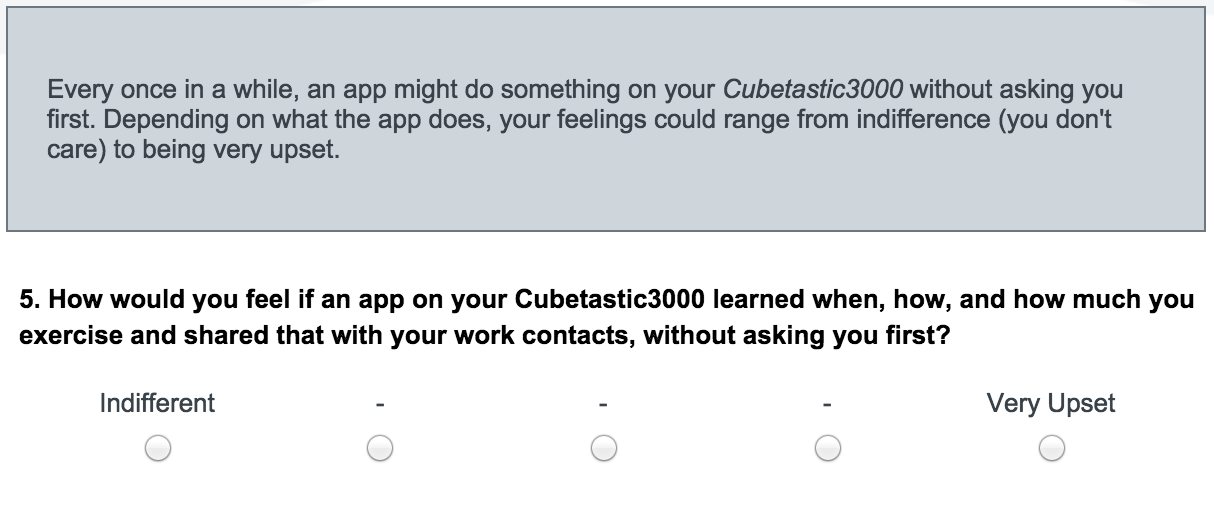
\includegraphics[width=\columnwidth]{images/prompt.png}
	\caption{An example of a wearable scenario question participants saw while taking the survey.}
	\label{fig:prompt}
\end{figure}

We combined 72 data types (<data>) with 4 data recipients (<recipient>) to form a pool of 288 scenarios (Table \ref{all-vur}). Each participant answered 6 questions that were randomly drawn from this pool, displayed in random order. We clarified for our participants that ``app'' meant the app's server, and that the data was not shared with anyone else. 

\subsubsection{Additional Questions}
The exit portion of the survey contained demographic questions (age, gender, and education), and then asked about wearable device ownership so we could control for prior exposure. An open-ended question on what would be the most likely risks associated with wearable devices was included to capture user concerns more broadly. To avoid biasing the open-ended question, we asked before concluding with the 10-question Internet Users' Information Privacy Concerns (IUIPC) index~\cite{malhotra2004internet}, which was included so we could control for participants' general privacy attitudes. However, we do realize that we asked this open-ended question after we had exposed our participants to a variety of wearables scenarios, which may have heightened their awareness of the possible risks. We talk about this more in Section 4. 

\subsection{Focus Group}
We conducted a one-hour focus group to validate our design, gauge comprehension, and measure fatigue. The focus group began with participants taking the survey then giving feedback on the format and the content, noting any instructions or questions that were unclear. The focus group concluded with a discussion of possible benefits and risks of wearable devices, in order to brainstorm any additional scenarios to include. Finally, we compensated participants with \$30 in cash. We recruited all of our focus group participants from Craigslist. Of the 13 participants, 54\% were female, and ages ranged from 18 to 64 ($\mu = 36.1$, $\sigma = 15.3$).  Education backgrounds ranged from high school to doctorate degrees, and professions included student, artist, marketer, and court psychologist.

\subsection{Recruitment and Analysis Method}
We recruited 2,250 participants over August 7--13, 2014 via Amazon's Mechanical Turk. We restricted participants to those over 18, living in the United States, and having a successful HIT completion rate of 95\% or above. We compensated each participant with \$1.75 upon successfully completing the survey. Based on incorrect responses to either of the two comprehension questions, we filtered out 366 (16\% of 2,250) participants. We filtered out an additional 99 participants (4\% of 2,250) due to incomplete responses, and three participants for being under 18, leaving us with a total sample size of 1,782. Of these, 57.9\% were male (1,031), 41.0\% were female (731), and 20 participants declined to state their genders. Ages ranged from 18 to 73, with a mean of 32.1 ($\sigma$ = 10.37). Almost half of our participants had completed a college degree or more (49.2\% of 1,782), which includes the 219 (12.3\% of 1,782) who reported graduate degrees. While our sample was younger and more educated than the U.S. population as a whole, we believe it is still consistent with the U.S. Internet-using population.

In performing our analysis in the next section, we chose to focus on the very upset rate (VUR) of each scenario~\cite{Felt}.  The VUR is defined as the percentage of participants who reported a `5' on the Likert scales. 
We use the VURs rather than the average of all Likert scores for the same reasons as Felt {\it et al.}: the VUR does not presume that the ratings, ranging from ``indifferent'' to ``very upset,'' are linearly spaced. Additionally, most people are likely to be upset, at least a little, in all scenarios, because a device is taking action without permission (rating distribution: ``1''= 759, ``2'' = 918, ``3'' = 1,452, ``4''' = 2,421, ``5'' = 8,344). Thus, the distinguishing factor is whether a participant was maximally upset. A limitation of this approach is that it only allows us to make {\it relative} comparisons between scenarios, rather than being able to definitively state how upset people might be if a single scenario were to occur.

\section{Results}
In this section, we present participants' responses to the various data-sharing scenarios, and discuss how and which various factors contributed to their risk perceptions. We had at least 141 responses per data type, 2,779 per recipient, and 35 responses per each unique data type/recipient combination. We conclude the section with participants' self-reported wearables concerns.\\

\noindent {\bfseries Data Type}
Based on our statistical models (later reported in Section \ref{sec:regression}), we observe that the largest effect on participants' VURs stemmed from the data being shared, rather than  with whom the data is shared. The most and least concerning data types are listed in Table \ref{top10-table}. 

Participants were most concerned about photos and videos, especially if they contained embarrassing content, nudity, or financial information. As seen in Table \ref{top10-table}, photos and videos accounted for five of the top ten concerns, and are almost unanimously considered to be concerning. Information that could be used to impersonate someone (e.g., usernames/passwords for websites), or photos of someone at home, were also among the most concerning data types. 

Participants were least concerned about data that could be collected through observations of public behavior, such as demographics (e.g., age, gender, language) or information available to advertisers (e.g., TV shows watched, music on device). As seen in Table \ref{top10-table}, participants' responses had a greater amount of variance.  This greater variance and overall decreased concern may be because of uncertainty with how the data would be used, or because the financial, social, or physical consequences would be less immediate.

Although certain data is considered unanimously upsetting to have shared, it is interesting to note that no data was considered unanimously non-upsetting to have shared, nor were there any data types that evoked strong disagreement between participants (i.e., bimodal). Generally, the average concern magnitude was inversely correlated with the standard deviation, which suggests the presence of ceiling effects for the most concerning data types. For the complete ranked list of data types in this study, see Table \ref{all-vur}.\\

\begin{table*}[t]
\begin{center}
\small
\begin{tabular}{| r | l | r | r |c |}
\hline
Rank & Data & VUR & $\sigma$ & Distribution \\
\hline
1 & video of you unclothed & 95.97\% & 0.31 & 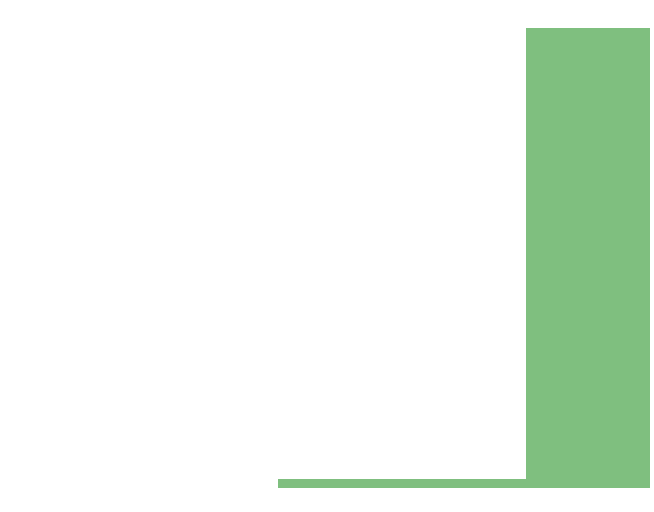
\includegraphics[width = 2cm, height = 0.5cm]{tex-inputs/data10/tookavideoofyouunclothedcombined} \\
2 & bank account information & 95.91\% & 0.35 & 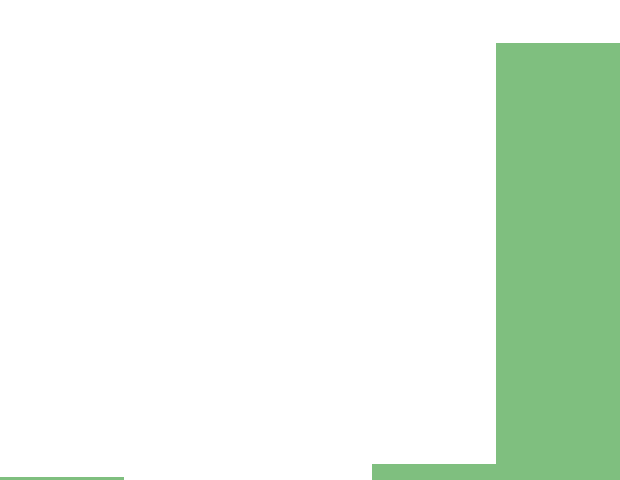
\includegraphics[width = 2cm, height = 0.5cm]{tex-inputs/data10/learnedyourbankaccountinformationcombined}  \\
3 & social security number & 94.84\% & 0.26 & 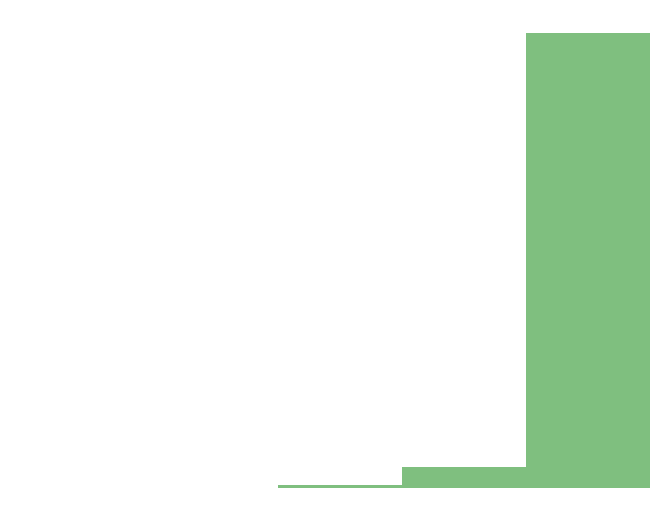
\includegraphics[width = 2cm, height = 0.5cm]{tex-inputs/data10/learnedyoursocialsecuritynumbercombined}\\
4 & video entering in a PIN at an ATM & 92.67\% & 0.47 & 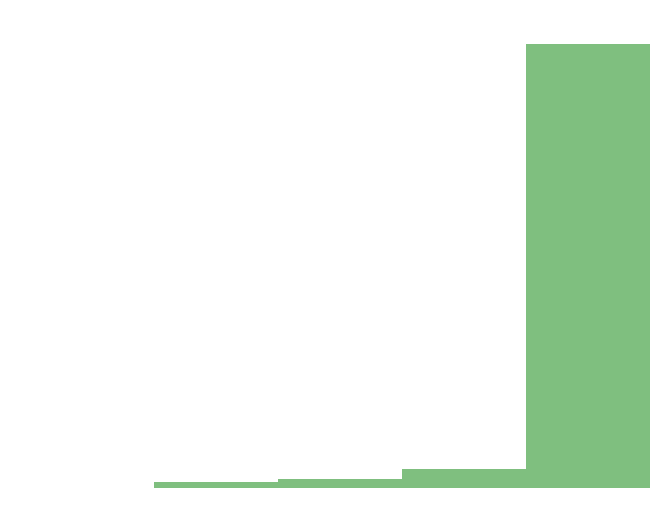
\includegraphics[width = 2cm, height = 0.5cm]{tex-inputs/data10/tookavideoofyouenteringinyourPINatanATMcombined}\\
5 & photo of you unclothed & 92.59\% & 0.46 & 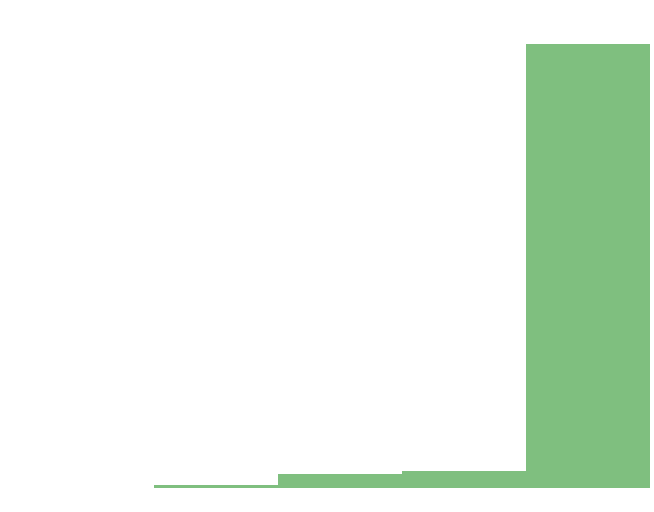
\includegraphics[width = 2cm, height = 0.5cm]{tex-inputs/data10/tookaphotoofyouunclothedcombined}\\
6 & photo of you that is very embarrassing & 91.39\% & 0.55 & 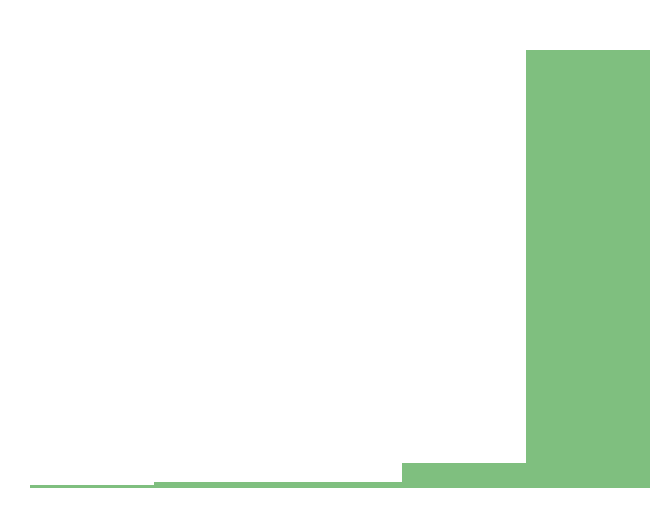
\includegraphics[width = 2cm, height = 0.5cm]{tex-inputs/data10/tookanincriminatingphotoofyoudoingsomethingembarrassingcombined}\\
7 & username and password for websites & 89.55\% & 0.62 & 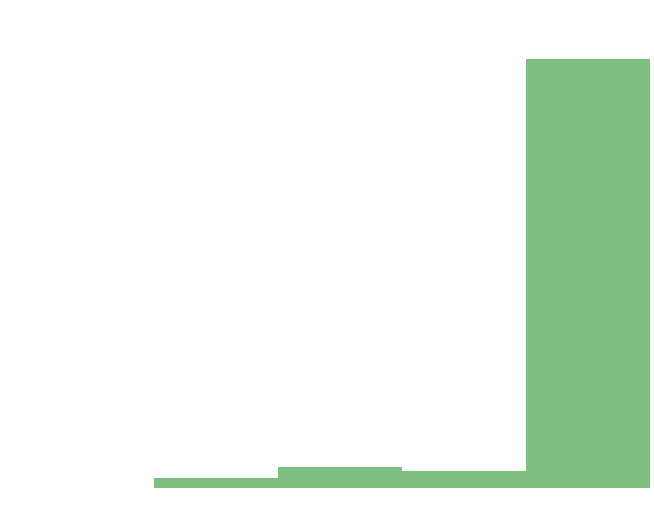
\includegraphics[width = 2cm, height = 0.5cm]{tex-inputs/data10/learnedyourusernameandpasswordforwebsitescombined}\\
8 & credit card information & 88.98\% & 0.56 & 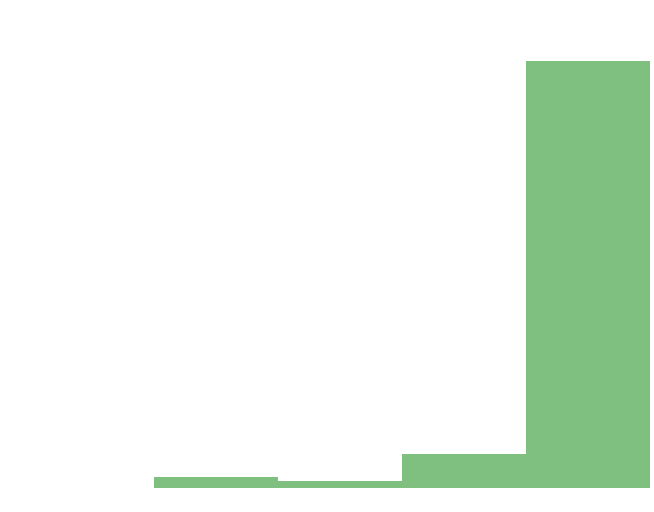
\includegraphics[width = 2cm, height = 0.5cm]{tex-inputs/data10/learnedyourcreditcardinformationcombined}\\
9 & video of you that is very embarrassing & 88.41\% & 0.53 & 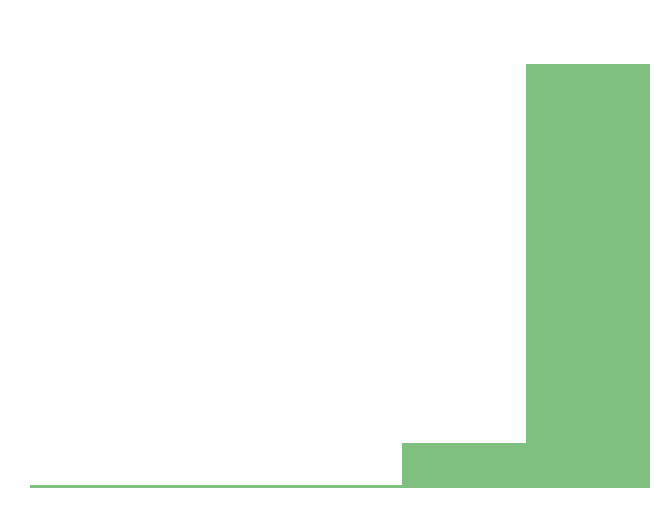
\includegraphics[width = 2cm, height = 0.5cm]{tex-inputs/data10/tookanincriminatingvideoofyoudoingsomethingembarrassingcombined}\\
10 & photo of you at home & 87.50\% & 0.60 & 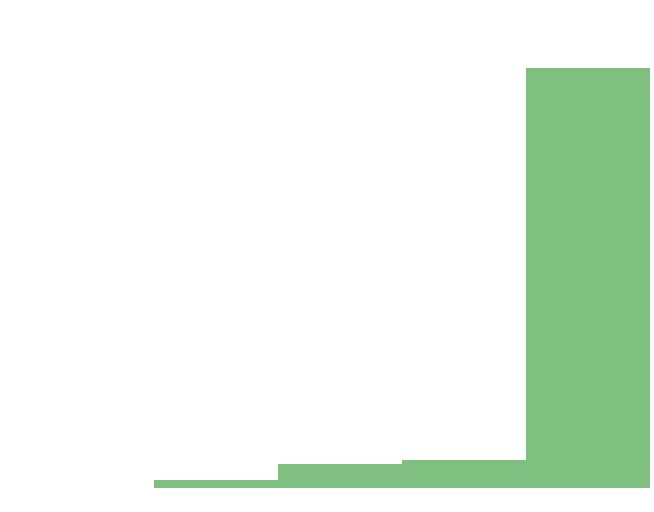
\includegraphics[width = 2cm, height = 0.5cm]{tex-inputs/data10/tookphotosofyou(withaninward-facingcamera)athomecombined}\\
 & \vdots & & & \\
64 & eye patterns (for eye tracking) & 40.51\%& 1.27 & 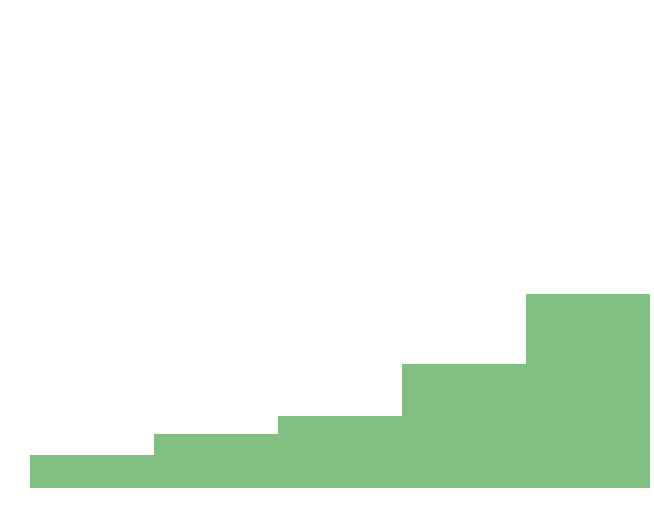
\includegraphics[width = 2cm, height = 0.5cm]{tex-inputs/data10/scannedyoureyetolearnyoureyepatterns(foreyetracking)combined} \\
65 & exercise patterns  & 38.66\% & 1.26 & 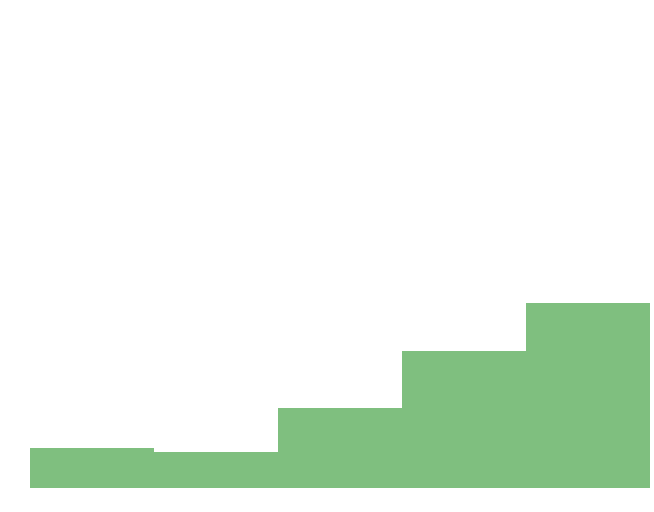
\includegraphics[width = 2cm, height = 0.5cm]{tex-inputs/data10/learnedwhenhowandhowmuchyouexercisecombined}\\
66 & when you are happy or having fun  & 34.75\% & 1.27 & 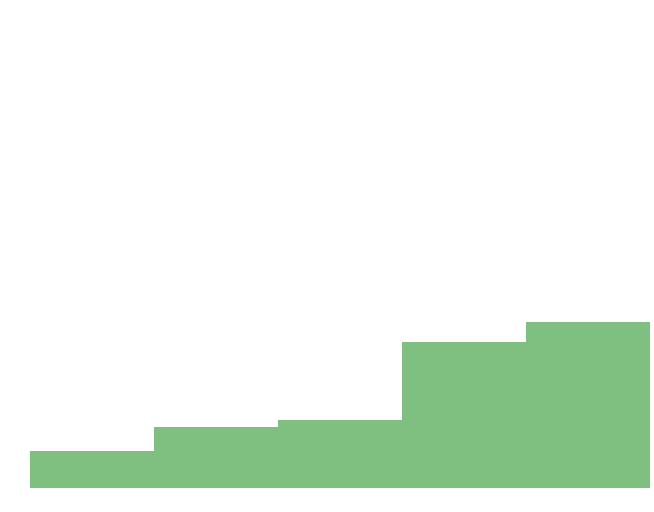
\includegraphics[width = 2cm, height = 0.5cm]{tex-inputs/data10/learnedwhenyouwerehappyorhavingfuncombined}\\
67 & television shows watched & 30.20\% & 1.40 & 
\includegraphics[width = 2cm, height = 0.5cm]{tex-inputs/data10/learnedwhattelevisionshowsyouwatchcombined}\\
68 & when you are busy or interruptible  & 29.50\% & 1.26 & 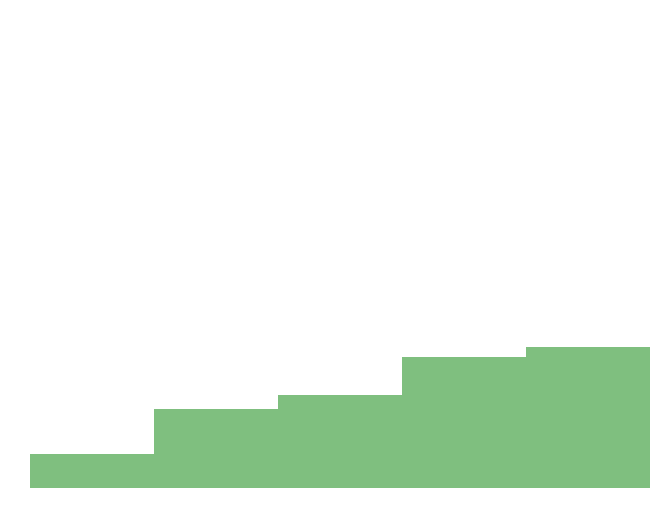
\includegraphics[width = 2cm, height = 0.5cm]{tex-inputs/data10/learnedwhenyouarebusyorinterruptiblecombined}\\
69 & music on device  & 28.06\% & 1.43 & 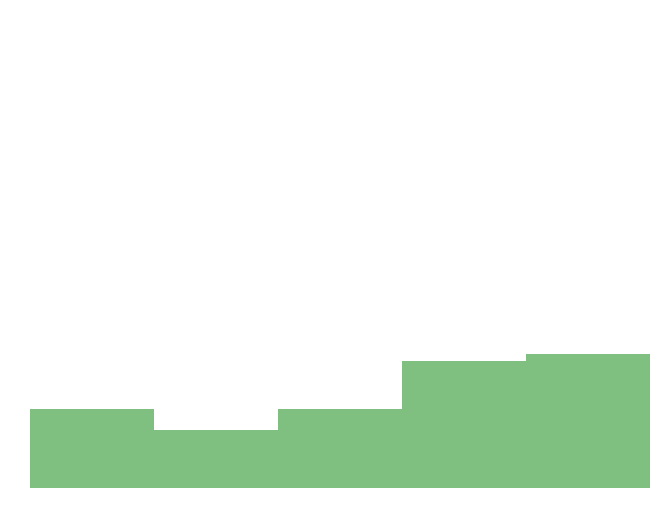
\includegraphics[width = 2cm, height = 0.5cm]{tex-inputs/data10/copiedanduploadedmusicfromyourdevicecombined}\\
70 & your heart rate & 27.50\% & 1.40 & 
\includegraphics[width = 2cm, height = 0.5cm]{tex-inputs/data10/learnedyourheartratecombined} \\
71 & age & 24.29\% & 1.43 & 
\includegraphics[width = 2cm, height = 0.5cm]{tex-inputs/data10/learnedyouragecombined}\\
72 & language spoken & 15.86\% & 1.49 & 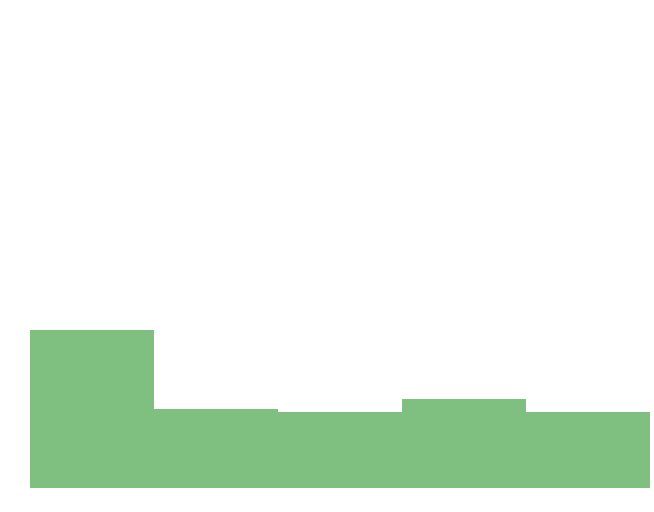
\includegraphics[width = 2cm, height = 0.5cm]{tex-inputs/data10/learnedthelanguageyouwerespeakingcombined}\\
73 & gender & 15.00\% & 1.45 & 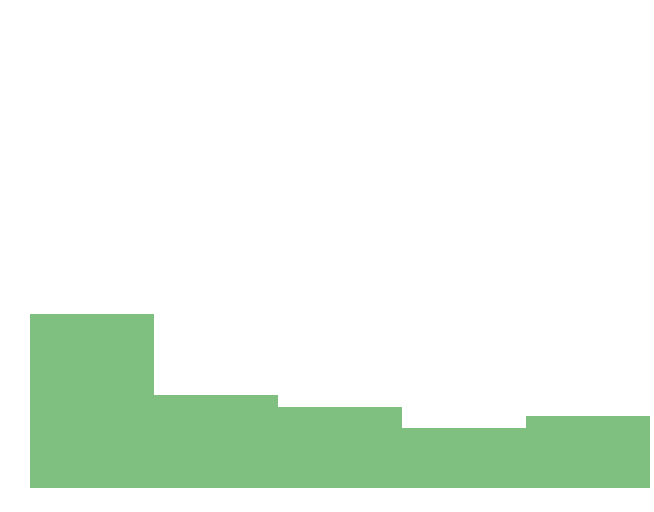
\includegraphics[width = 2cm, height = 0.5cm]{tex-inputs/data10/learnedyourgendercombined}\\ 
\hline
\end{tabular}
\caption{The 10 most and least upsetting data types, across all recipients.}
\label{top10-table}
\end{center}
\end{table*}

%A statistical analysis regarding the significance and confidence of <data> types with respect to all 72 was not performed due to the space constraints of the paper. We do consider all <data> categories in our statistical model, which provides an analysis of what factors had contributed to the perceived severity of a particular situation. 

\noindent {\bfseries Data Recipient}
A statistically significant difference in VUR exists between data shared with an application versus human recipients. On average, 42\% of participants stated that they would be ``very upset'' if their data was shared with only an application's servers, whereas the VURs for friends (70\%), work contacts (75\%), and the public (72\%) were almost double (Table \ref{recipient-vur}). A chi-square test indicated that these differences were statistically significant (Table \ref{recipient-chi}). However, these effect sizes were small: the largest effect was between work contacts and an app's server ($\phi=0.11$); while the VUR for sharing with work contacts was significantly higher than sharing with friends, the effect size was negligible ($\phi=0.004$). 

The statistical significance arises for two distinct reasons. Firstly, sharing data only with an application's server carries less social impact. And for our participants, it may seem that it is shared with fewer people. Additionally, there is a class of data which may be considered odd for a human to know, but completely normal for a wearable device to know (e.g., it's okay if your Fitbit knows when you sleep, but maybe less so for your friends).

We note that this chi-square test violates the assumption of independent observations, since participants responded to multiple scenarios with multiple recipients. But based on the randomization of treatments and large sample size, we do not believe that this significantly impacted our results. Similarly, we are unaware of a more appropriate test, given our data format. Cochran's Q requires binary outcomes (i.e., participants would have had to answer only one question for each data recipient, preventing us from adequately controlling for data type) and a repeated measures ANOVA requires normality (our data was not normally distributed). Nonetheless, we repeated our analysis using only one randomly-selected data point per participant and found that our selected test was robust to this violation. Therefore, we conclude that participants were significantly more concerned about having their data seen by a human versus an application, though differences between specific human groups such as the public, friends, and work contacts were not as significant. Our results motivate mechanisms for data taint tracking and accidental data sharing prevention.

However, we do not claim that there are no distinctions between the friends, public, and work contact recipients. People are more comfortable sharing certain data types with certain human recipients. For instance, participants were significantly more uncomfortable sharing if they were lying, nervous, or stressed to work contacts compared to the rest of the data recipients. Table \ref{all-vur} shows the complete VURs and rankings of all data types by recipient.\\

\begin{table}[t]
\begin{center}
\small
\begin{tabular}{| r | l | r | l |c |}
\hline
Rank & Recipient & VUR & sigma & Distribution \\
\hline
1 & Work Contacts & 75.16\% & 0.94 & 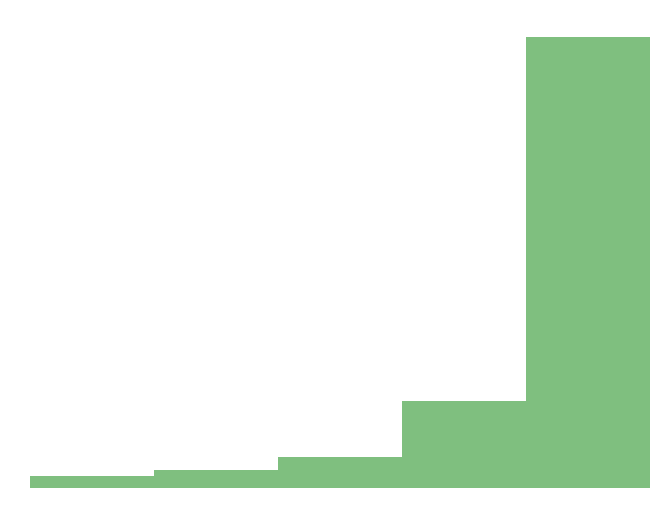
\includegraphics[width = 2cm, height = 0.5cm]{tex-inputs/recipient4/recipient_work} \\
2 & Public & 72.41\% & 0.98 & 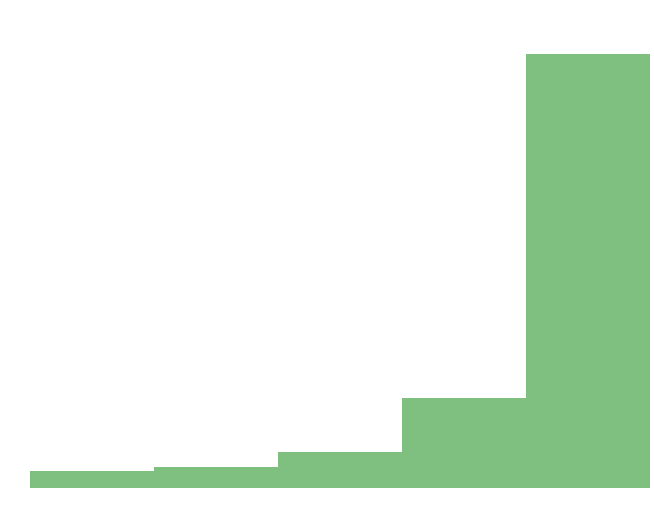
\includegraphics[width = 2cm, height = 0.5cm]{tex-inputs/recipient4/recipient_pub}  \\
3 & Friends & 69.47\% & 1.02 & 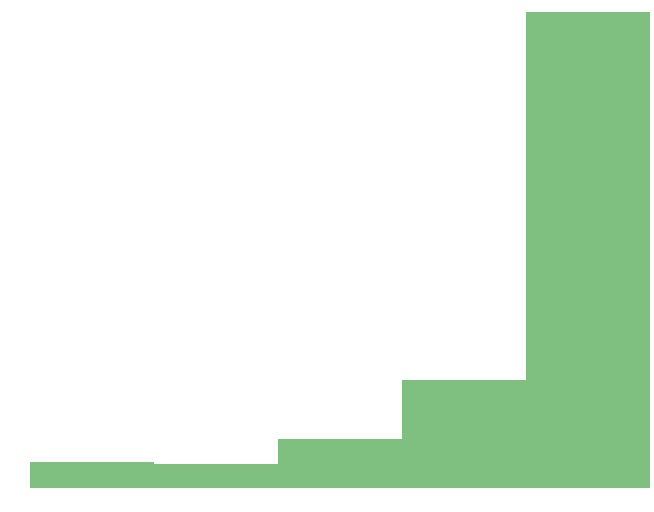
\includegraphics[width = 2cm, height = 0.5cm]{tex-inputs/recipient4/recipient_friends}\\
4 & App's Server & 42.28\% & 1.15 & 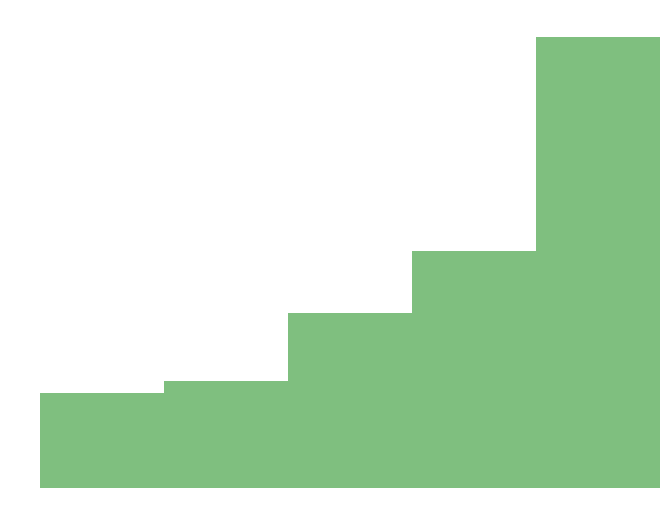
\includegraphics[width = 2cm, height = 0.5cm]{tex-inputs/recipient4/recipient_app}\\
\hline
\end{tabular}
\caption{The overall upset rate for all recipients.}
\label{recipient-vur}
\end{center}
\end{table}

\begin{table}[t]
\small
\begin{center}
\begin{tabular}{|l|r|r|r|r|}
\hline
Recipients	& $\chi^2$ & p-value 	& n & $\phi$ \\
\hline
Work-App	& 565.910 & <0.0001 & 5,083 & 0.111\\
Public-App	& 481.776 & <0.0001 & 5,1988& 0.093\\
Friends-App & 381.653 & <0.0001 & 5,096 & 0.075\\
Friends-Work & 20.39 & <0.0001 & 5,037 & 0.004\\
Friends-Public & 5.41 & <0.0200 & 5,142 & 0.001\\
Work-Public&  5.00 & <0.0253 & 5,129	& 0.001\\
\hline
\end{tabular}
\caption{Results of a chi-square test to examine VUR based on data recipient, across all data points.}
\label{recipient-chi}
\end{center}
\end{table}

\noindent {\bfseries Open-ended Concerns}
We captured participants' reactions to wearable devices as a whole by asking the following open-ended question:

\begin{quotation}
\noindent
\textit{What do you think are the most likely risks associated with wearable devices?}
\end{quotation}

The participants were presented with a blank box to write in, with no particular suggestion on what to talk about, and with no character limit to their open-ended responses. Table \ref{openresponses} shows common user concerns related to wearable devices. Appendix \ref{sec:coding} details the responses categorized in each coding label. Note that participants were especially concerned with privacy and security, however, we do realize that we asked this open-ended question after we had exposed our participants to a variety of privacy-related scenarios, which may have heightened their awareness of the possible privacy and security risks. 

\begin{quotation}
\noindent
\textit{P246: ``Privacy and security of your data, particularly for eg, [sic] stored financial/payment or medical information''}\\

\noindent
\textit{P1256: ``They can be hacked and then your security will be compromised.''}
\end{quotation}

Other significant concerns included being unaware of what the device is collecting, doing, or which information it is using (Being Unaware), long-term health effects caused from wearing the device such as cancer from EMF waves (Health), and safety hazards from wearing the device, such as distractions that cause car accidents (Safety).

\begin{quotation}
\noindent
\textit{P1742: Capturing and sharing data and information that you are unaware of.}\\

\noindent
\textit{P670: ``Are there microwaves or some such type of waves that can pass through the brain and harm the brain?  Wearing something all day can hurt that area of the body after a while.''}\\

\noindent
\textit{P1038: ``Becoming distracted by the devices while doing other activities that require concentration such as driving.''}\\

\end{quotation}

Interestingly, a modest amount of participants were also concerned with resulting changes in social behaviors, such as dependence on devices or spending less time with loved ones (Social Impact). 

\begin{quotation}
\noindent
\textit{P1425: I think the biggest risk is how they may effect society as a whole... a wearable technology that's always on and available may push things even further to the point where people spend less time actually interacting with loved ones, and applying their own critical thinking in certain situations, instead always relying on their devices.}
\end{quotation}

The landscape of users' perceived risks associated with wearable devices is broad, encompassing concepts such as privacy and security, but also non-technical aspects such as health, safety, and change in social behaviors. We hope that this motivates researchers to investigate these aforementioned risks. \\

\begin{table}[t]
\begin{center}
\begin{tabular}{|l|r|r|}
\hline
Concern &  Responses &  Frequency   \\
\hline
Privacy & 452 & 25.32\% \\
Being Unaware & 275 & 15.40\% \\
%Unaware Use & 167 & (9.36\%)\\
%Unaware Collection & 64 & (3.59\%)\\
%Unaware Access & 44 & (2.46\%)\\
Health Risk & 191 & 10.70\%\\
Safety & 185 & 10.42\%\\
Social Impact &	157 & 8.80\%\\
Financial Cost & 151 & 8.46\%\\
Security &	144 & 8.07\%\\
Accidental Sharing &	69 & 3.87\%\\
Miscellaneous &	57 & 3.19\%\\
None	& 51 & 2.86\%\\
Social Stigma &	39 & 2.18\%\\
False Information & 33 & 1.85\%\\
Don't know & 31 & 1.74\%\\
Aesthetics 	& 19 & 1.06\%\\
Don't care 	& 11 & 0.62\%\\
\hline
\end{tabular}
\caption{The most common open-ended risks associated with owning a wearable device.}
\label{openresponses}
\end{center}
\end{table}

\noindent {\bfseries Demographics Factors}
We see that privacy is a main concern for wearables users. Additionally, we show that privacy preferences should also be a consideration when configuring a user's device. A participant's self-reported level of privacy concern---as determined by the IUIPC scale~\cite{malhotra2004internet}---is the biggest demographic predictor of VURs. A Spearman correlation yielded a statistically significant effect between average IUIPC scores and average VUR ($\rho=0.446$, $p<0.0005$), which suggests responses to questions were mostly based on privacy preferences. Additionally, we observed that age was another significant predictor of VUR ($\rho=0.121$, $p<0.0005$), but we suspect that this effect is due to the significant correlation between age and IUIPC scores ($\rho=0.188$, $p<0.0005$). Others have observed that older individuals tend to be more privacy protective~\cite{varian2005demographics}.

While we initially observed an effect on VURs based on whether or not participants claimed to already own wearables (57.0\% vs. 60.8\%, respectively; Mann-Whitney $U=202,896$, $p<0.032$), this difference did not remain significant upon correcting for multiple testing (Bonferroni corrected $\alpha=0.01$). The effect of a participant's gender also did not remain significant upon correcting for multiple testing. We observed no correlation between a participant's education level and VUR.\\

\noindent {\bfseries Regression Models}
\label{sec:regression}
To examine the relative effect of each factor on participants' VURs, we constructed several statistical models to predict whether a participant would be ``very upset'' with a given scenario based on the data type, data recipient, and their demographic factors (i.e., age, education, gender, and privacy attitudes). We performed binary logistic regressions using generalized estimating equations, which account for our repeated measures experimental design (i.e., each participant contributed multiple data points).

\begin{table}[t]
\centering
\begin{tabular}{|l| r| r| r|}
\hline
Parameters & $\chi^2$ & $df$ & QIC\\
\hline
\hline
(Intercept) & 423.96 & 1 & 13,209.1\\
\hline
(Intercept) & 207.07 & 1 & 12,551.49\\
IUIPC (covariate) & 368.5 & 1 & \\
Gender (covariate) & 6.30 & 1 & \\
\hline
(Intercept) & 411.66 & 1 &12,458.86\\
Data Recipient & 599.72 & 3 & \\
\hline
(Intercept) & 418.02 & 1 & 11,382.75\\
Data Type & 1,141.40 & 71 & \\
\hline
(Intercept) & 66.18 & 1 & 9,609.65 \\
Data Recipient & 617.25 & 3 & \\
Data Type & 1,288.51 & 71 & \\
IUIPC (covariate) & 105.73 & 1 & \\
Gender (covariate) & 9.74 & 1 & \\
IUIPC $\times$ Gender & 8.33 & 1 &\\
\hline
\end{tabular}
\caption{Goodness-of-fit metrics for various binary logistic models of our data using general estimating equations to account for repeated measures. The columns represent the Wald test statistic for each parameter and the overall Quasi-Akaike Information Criterion (QIC) for each model. Each parameter listed was statistically significant at $p<0.005$.}
\label{regression}
\end{table}

We created several models using two independent variables as predictors: data and recipient. This resulted in a total of 72 types of data shared with 4 possible recipients. Demographic factors used as covariates are: age, gender, education, wearable device ownership (yes/no), and mean IUIPC score. For each model, we performed Wald's test to examine the model effects attributable to each of these parameters. The only covariates that had an observable effect on our models were participants' gender and IUIPC scores, which also exhibited an interaction effect with each other. Thus, we opted to remove the other covariates from our analysis. Table \ref{regression} shows the various models that we examined and the Quasi-Akaike Information Criterion (QIC), which is a goodness-of-fit metric for model selection that also accounts for complexity (lower relative values indicate better fit). As shown, the type of data being shared (data type) was found to be the strongest predictor of a high VUR.

While these models illustrate the relative weights that users place on information when determining a scenario as truly upsetting, one shortcoming of this approach is its generalizability: the data predictor is categorical and limited to the data that we specifically chose for this study. To make our data set more generalizable to other use cases, we coded each data type in two ways: in terms of broad descriptions of the type of data (e.g., video, audio, etc.) and the type of risk it presents. Two researchers agreed on a codebook and independently coded each of the 72 data types.\\

The data types fell into these six categories:

\begin{enumerate}[topsep=0pt,itemsep=-1ex,partopsep=1ex,parsep=1ex]
\item Photo
\item Video
\item Audio
\item Behavioral Information
\item Biometric Information
\item Demographic Information
\end{enumerate}

While the first three categories are self-explanatory, the latter three categories are all based on different user characteristics. We defined {\it behavioral information} as observations about the user's activities; {\it biometric information} as measurements of the user's body; and {\it demographic information} as non-biometric information about the user's traits. \\

The risks for data types fell into these five categories:

\begin{enumerate}[topsep=0pt,itemsep=-1ex,partopsep=1ex,parsep=1ex]
\item {\bf Financial:} the loss of money or property.
\item {\bf Image:} the loss of control over one's self-image (e.g., publicizing something embarrassing).
\item {\bf Medical:} the disclosure of medical information.
\item {\bf Physical:} physical harm to the user.
\item {\bf Relationships:} damage to the user's inter-personal relationships.
\end{enumerate}

After independently coding, the researchers met to resolve any disagreements, such that the results reflect unanimity. There was  83\% agreement prior to resolution. Cohen's $\kappa$ was 0.81 for the data categories and 0.75 for the  risk categories, both indicating ``excellent'' agreement~\cite{Fleiss2003}. 

With regard to data types, the most concerning type of data is video (78.0\%), which was ranked similarly to photos (76.2\%). Next are audio (66.8\%) and demographic data (65.4\%), followed by behavioral (53.1\%) and biometric (46.3\%) data. We suspect that demographic data was more concerning because it included information such as a Social Security Number, bank account information, and other financial information. We chose to categorize them as such as they are non-biological descriptors of the user. We were very surprised that biometric information was seen as relatively benign compared to the other broad categories of data. One hypothesis is that since most home users do not use biometric authentication, they may have an inaccurate understanding of the types of systems that might be at risk if biometric data is stolen and abused.

With regard to the presented risks, we observed that average VURs were highest for financial information disclosure (82.0\%). Information regarding relationships (69.2\%), physical safety (66.4\%), and self-image (65.8\%) followed. VURs were lowest for medical information disclosure (47.4\%). One reason why medical risks were ranked relatively low is that this category broadly covered scenarios involving data about the user's health, but also included more basic medical information, such as age, gender, and emotional state. As mentioned earlier, participants saw these as publicly observable and therefore unconcerning.


\begin{table}[t]
\centering
\begin{tabular}{|l| r| r| r|}
\hline
Parameters & $\chi^2$ & $df$ & QIC\\
\hline
\hline
(Intercept) & 442.66 & 1 & 12,727.42\\
Risk & 405.18 & 4 & \\
\hline
(Intercept) & 380.39 & 1 & 12,681.86\\
Data Category & 439.45 & 5 & \\
\hline
(Intercept) & 256.15 & 1 & 12,061.87\\
Risk & 157.84 & 4 & \\
Data Category & 183.90 & 5 & \\
Risk $\times$ Data Category & 259.81 & 8 & \\
\hline
(Intercept) & 62.65 & 1 & 10,406.35\\
Risk & 205.21 & 4 & \\
Data Category & 250.35 & 5 & \\
Recipient & 546.89 & 3 & \\
IUIPC (covariate) & 103.94 & 1 & \\
Gender (covariate) & 9.80 & 1 & \\
IUIPC $\times$ Gender & 8.21 & 1 & \\
Risk $\times$ Data Category & 303.44 & 8 & \\
Recipient $\times$ Risk & 39.14 & 12 & \\
\hline
\end{tabular}
\caption{Metrics for additional binary logistic models of our data using general estimating equations to account for repeated measures. The columns represent the Wald test statistic for each parameter and the overall Quasi-Akaike Information Criterion (QIC) for each model. Each parameter listed was statistically significant at $p<0.005$.}
\label{regression2}
\end{table}

Using these two new variables as additional independent variables (and removing the previous data type variable), we created a second set of models. Because these risk categories and mediums are less likely to change over time, models that take these into account are likely to be more useful and less likely to be overfit. What these models show us is that both risk and medium are relatively strong predictors by themselves, and have an even stronger interaction effect. When the data recipient and covariates are added to the model, the resulting goodness-of-fit is not much worse than that of the model using the actual data type. 

\section{Discussion}

\noindent {\bfseries Limitations}
One of the limitations of our experiment is that our participants might not have knowledge or interest in wearables and their capabilities; 83\% of our participants reported that they do not own a wearable. Because of this, our participants may be over or underestimating the risk, stemming from an unawareness of what can be inferred from the data, not having clear relations of new technology with respect to familiar ones, and a higher likelihood of being influenced by reports of recent events.\footnote{At the time of the survey, stories of exploding batteries were in the news~\cite{1_levin_2014}, which were explicitly reported as a concern in our open-ended question.}  For instance, biometrics were generally not a concern for our participants, although there are many security and privacy implications~\cite{prabhakar2003biometric}. Our participants also did not differentiate between the benefits and risks of various new capabilities.

We recruited both wearable users and non-users in order to yield a more representative sample of the general population. We could have easily recruited only wearables owners or people specifically interested in wearables. However, that would have its own biases and limitations. At the time of this writing, about 85\% of the general population do not own wearable devices~\cite{Nilsen,WearableStatNews}, indicating our study is reflective of the current population. 

Because of the privacy paradox, participants' stated responses may differ from how they may react to these same scenarios in real life~\cite{norberg2007privacy, jensen2005privacy}. At the same time, our results do reflect actual perceptions of wearable devices and the associated privacy scenarios involving them. This is an unavoidable, yet important distinction to make with of studies of this nature: our primary goal was to examine perceptions and preferences, so that future systems can be designed with these in mind. We do not expect that such systems will satisfy users in all situations, however, we believe that user-centered design will still be a vast improvement over {\it post hoc} approaches (or ignoring user concerns altogether). 

Although we presented our participants with a prompt illustrating all the benefits of a wearable device, the questions we asked isolated the risk from the benefits of sharing data with a particular recipient. We sacrificed context due to the complexity of the question necessary for the participant to answer correctly. Users are willing to tolerate risks if there is enough benefit associated with that risk. We do believe that since all of our questions were out of context, our study does represent what data people ambiguously would like to be private and secure, and is accurate for measuring user perceptions of wearables.\\

\noindent {\bfseries Future Research Directions}
We find that although people have opinions on applications which are familiar, users do not know the risk associated with new data or unfamiliar applications. We hope our work both informs the direction for future research to secure video, audio, and other currently considered sensitive sensor input channels, but also encourages work for contextual and user-input-independent permission models and access control schemes.

Further work can be done to expand various aspects of this study. Investigating more fine-grained data types (e.g., investigating specific instances of location data, versus location data in general) would be a useful endeavor to gain further insight into user perceptions. Adding additional recipients, such as ``advertisers'' or ``acquaintances'' may lead to more nuanced results. Additionally, the open-ended concerns illuminate areas of possible future research, such as the design of a distraction-free interface to prevent safety issues, and how to minimize negative social impact. 

\section{Related Work}
\noindent {\bfseries Ubiquitous Sensing} We are rapidly moving towards a world of ubiquitous sensing and data capture, with ensuing privacy challenges~\cite{abowd2000charting,palen2003unpacking,camp2000internet}. Roesner {\it et al.}\ urge the community to address potential concerns for wearable devices before the technologies become widespread~\cite{roesner2014security} and explore the unique and difficult problems these devices present in terms for law and policy~\cite{roesner2014augmented}. Many researchers have worked to study how privacy can be preserved in the presence of ubiquitous devices. Examples of such efforts include frameworks to design for privacy~\cite{bellotti1993design,camp2003designing,langheinrich2001privacy}, protocols for anonymous communication~\cite{cornelius2008anonysense}, evaluation metrics for privacy~\cite{scholtz2004toward}, and privacy models~\cite{hong2004privacy, jiang2002approximate}. Our work aims to augment works like these with an understanding of what privacy means to the end user. \\

\noindent {\bfseries Lessons from Smartphones} Smartphones allow applications to access new types of data. While this tends to benefit users, they do not think of the privacy implications. Lindqvist {\it et al.}\  studied a popular location tracking application, and found that people share their location information for gaming, signaling availability to friends, without concern for the privacy implications of broadcasting that information~\cite{lindqvist2011m}. There are still many unresolved concerns such as the opaqueness that prevents users from fully understanding how applications are using their data or rogue applications inappropriately accessing data~\cite{1_kane_2010, zhou2011taming}.

Felt \etal previously studied the security concerns of smartphone users by conducting a large-scale online survey~\cite{Felt}. Their survey asked 3,115 smartphone users about 99 risk scenarios. Participants were asked how upset they would be if a certain action occurred without their permission. Participants rated each situation on a Likert scale ranging from ``indifferent (1)'' to ``very upset (5).'' Our methodology closely follows that study, but with scenarios chosen to shed light on the security and privacy risks of wearable devices.\\

\noindent {\bfseries User Perceptions} While risk communication for the physical world has been examined for several decades (e.g.,~\cite{Fischhoff,Morgan2001}), research into effectively communicating computer-based risks has only recently been researched. For example, both Garg {\it et al.}\ and Blythe {\it et al.}\ show that due to varying perceptions and abilities that correlate with demographic factors, computer-based risk communication should employ some degree of demographic targeting~\cite{Garg2012,Blythe2011}. While this work is likely applicable to wearable computing risk communication, we believe that a better understanding of users' risk perceptions in this domain is warranted, prior to examining risk communication.

One limitation of user perceptions is that people do not always have enough information to make privacy-sensitive decisions. Even if users did have this information, it has been shown that users often trade off long-term privacy for short-term benefits~\cite{acquisti2005privacy}. Furthermore, actual behavior may deviate from stated privacy preferences~\cite{spiekermann2001privacy}. However, understanding user concerns is a necessary first step not only for risk communication, but preventative measures in general against breaches of privacy and security in a new threat landscape. 

\section{Conclusion}

 Our survey of 1,784 Internet users is the first large-scale study to investigate user-centric security and privacy concerns for wearable devices. We contribute a comprehensive ranking of possible risks associated with wearable devices, across various recipients. Our open-ended responses show that privacy and security are at the top of user's overall concerns. While wearables are still in their infancy, perceptions of situations and capabilities are likely to change rapidly with advancements and increased exposure. However, there has not been much prior work done to determine which threats in the emerging threat landscape are pertinent to focus on. Our examination of possible data concerns agree with previous studies of smartphone users that found that video capture and financial data are the most sensitive data types. Various systems which detect and take actions for sensitive objects in photos and videos will be critical as wearables and other devices become more ubiquitous. We also found that users' self-reported privacy preferences are correlated with how they may react, even with respect to situations that they are unfamiliar with. Our results may be used by system designers to create permissions and access control mechanisms that do not directly depend on users' inputs. We hope that this work has given a comprehensive overview of user concerns and informs designs of future privacy and security work for wearable devices. 

\bibliographystyle{abbrv}
\bibliography{bibliography.bib} 

%!TEX root = ../paper.tex
\appendix

\section{Fischhoff Prompts}
\label{sec:prompt} 

\textit{We would like to ask you to rate the <risks/benefits> associated with each of the following technologies.}

{\bf Risks:} \textit{Consider all types of risks: the risk of physical harm or death, the risk to others or bystanders, the financial cost of the technology, any distress caused by the technology, what the consequences would be if the technology was misused, any impact on the public, work, or personal life, and other considerations. (e.g. for electricity, consider the risk of electrocution, the pollution caused by coal, the risk that miners need to take to mine the coal, the cost to build the infrastructure to deliver electricity, etc.) Give a global estimate over a long period of time (say, a year) of both intangible and tangible risks.} 

\textit{Do not consider the costs or risks associated with these items. It is true, for example, that sometimes swimmers can drown. But evaluating such risks is not your present job. Your job is to assess the gross benefits, not the net benefits which remain after the costs and risks are subtracted out.}

\textit{Please rate the following technologies below with a number. We know that this might be a bit hard to do, but please try to be as accurate as possible, adjusting the numbers until they feel they are right for you. Start with the least risky technology at 10 and assign higher numbers for the more risky technologies. (For instance, a technology rated 14 is half as risky as a technology rated 28.)}

{\bf Benefits:} \textit{Consider all types of benefits: how many jobs are created, how much money is generated directly or indirectly, how much enjoyment is brought to people, how much a contribution is made to the people's health and welfare, what this technology promotes, and so on. (e.g. for swimming, consider the manufacture and sale of swimsuits, the time spent exercising, the social interactions during swimming, and the sport created around the activity.) Give a global estimate over a long period of time (say, a year) of both intangible and tangible benefits.}

\textit{Do not consider the costs or benefits associated with these items. It is true, for example, that electricity also creates a market for home appliances. But evaluating such benefits is not your present job. Your job is to assess the gross risks, not the net risks which remain after the costs and risks are subtracted out.} 

\textit{Please rate the following technologies below with a number. We know that this might be a bit hard to do, but please try to be as accurate as possible, adjusting the numbers until they feel they are right for you. Start with the least beneficial technology at 10 and assign higher numbers for the more beneficial technologies. (For instance, a technology rated 34 is twice as beneficial as a technology rated 17.)}

\section{Coding Label Definitions}
\label{sec:coding}
Researchers coded the self reported answers as follows:\\
{\bf Privacy}: ``privacy,'' mention of personal details, spying. \\
{\bf Security}:  ``security,'' mention of malware, hacking. \\
{\bf GPS tracking}: ``location,'' ``GPS,'' mention of monitoring. \\
{\bf Being Unaware}: mention of using, collecting, and disclosing data without permission. \\
{\bf False information}: inaccurate or maliciously false data.\\
{\bf Health Risk}: mention of radiation, cancer, or other effects.\\
{\bf Safety}: mention of distractions causing car crashes and injuries, violence due to the device, injuries from malfunctions.\\
{\bf Discomfort}: mention of eye strain, headache, irritation. \\
{\bf Financial cost}: cost of buying or using the device. \\
{\bf Theft}: mention of device theft. \\
{\bf Social Impact}: mention of dependency, distance from people, changes in decision making, etc. \\
{\bf Social Stigma}: mention of judgment, hate, or bystanders.\\ 
{\bf Aesthetics}: mention of fashion or looking dorky. \\
{\bf Miscellaneous}: odd comments, uncommon concerns. \\
{\bf None}: ``None,'' mention of no threat, or no real concerns \\
{\bf Don't know}: ``do not know,'' general confusion \\
{\bf Don't care}: `` do not care,'' nonchalant answers 


%!TEX root = ../paper.tex

\section{Concern Factor: Recipient}
\label{sec:recipient-appendix} 

\begin{table*}[t]
\begin{center}
\small
\begin{tabular}{| l | r | r | r | r | r |}
\hline
Question & All & Friends & Public & Work& App \\
\hline
video of you unclothed & 95\% (1) & 97\% (4) & 94\% (10) & 100\% (1) & 90\% (2) \\ 
bank account information & 95\% (2) & 94\% (10) & 95\% (7) & 100\% (1) & 90\% (1) \\ 
social security number & 94\% (3) & 100\% (1) & 100\% (1) & 93\% (9) & 88\% (3) \\ 
video entering in a PIN at an ATM & 92\% (4) & 100\% (1) & 93\% (12) & 87\% (20) & 88\% (4) \\ 
photo of you unclothed & 92\% (5) & 96\% (6) & 91\% (16) & 100\% (1) & 77\% (6) \\ 
photo of you that is very embarrassing & 91\% (6) & 94\% (8) & 100\% (1) & 94\% (6) & 78\% (5) \\ 
username and password for websites & 89\% (7) & 96\% (5) & 95\% (9) & 94\% (7) & 64\% (14) \\ 
credit card information & 88\% (8) & 100\% (1) & 93\% (13) & 95\% (5) & 65\% (13) \\ 
video of you that is very embarrassing & 88\% (9) & 91\% (13) & 94\% (11) & 94\% (7) & 71\% (9) \\ 
photo of you at home & 87\% (10) & 85\% (19) & 96\% (5) & 93\% (10) & 71\% (10) \\ 
audio recording of work conversations & 86\% (11) & 94\% (9) & 96\% (6) & 100\% (1) & 53\% (24) \\ 
video of entering in a passcode to a door & 85\% (12) & 95\% (7) & 89\% (21) & 81\% (35) & 75\% (7) \\ 
audio recording of phone conversations & 85\% (13) & 93\% (11) & 97\% (4) & 90\% (14) & 56\% (20) \\ 
amount of money you have & 84\% (14) & 90\% (14) & 100\% (1) & 93\% (11) & 63\% (15) \\ 
video of you intoxicated & 83\% (15) & 81\% (26) & 91\% (16) & 88\% (17) & 68\% (11) \\ 
when you have sex & 81\% (16) & 78\% (31) & 87\% (23) & 90\% (15) & 73\% (8) \\ 
video of you at home & 81\% (17) & 87\% (16) & 86\% (24) & 89\% (16) & 60\% (17) \\ 
photo of you intoxicated & 78\% (18) & 80\% (27) & 90\% (18) & 87\% (23) & 53\% (25) \\ 
photo of you at random  & 78\% (19) & 82\% (24) & 83\% (29) & 81\% (32) & 66\% (12) \\ 
audio recording of conversations & 78\% (20) & 86\% (18) & 85\% (26) & 87\% (20) & 55\% (21) \\ 
medical conditions & 77\% (21) & 92\% (12) & 85\% (25) & 85\% (27) & 40\% (37) \\ 
video of you at random & 76\% (22) & 73\% (40) & 90\% (19) & 88\% (19) & 48\% (31) \\ 
video of you off-guard & 76\% (23) & 85\% (21) & 79\% (34) & 91\% (13) & 53\% (23) \\ 
photo of your work or workplace & 74\% (24) & 76\% (33) & 82\% (31) & 81\% (32) & 62\% (16) \\ 
username for websites & 73\% (25) & 90\% (15) & 74\% (43) & 84\% (28) & 50\% (29) \\ 
address & 72\% (26) & 62\% (50) & 93\% (14) & 81\% (31) & 51\% (28) \\ 
audio recording you captured & 72\% (27) & 87\% (17) & 75\% (40) & 72\% (46) & 50\% (29) \\ 
photo of you off-guard & 72\% (28) & 83\% (23) & 80\% (32) & 80\% (37) & 45\% (33) \\ 
photo downloaded from internet & 71\% (31) & 79\% (29) & 76\% (38) & 86\% (25) & 32\% (47) \\ 
photo others sent you & 71\% (32) & 85\% (21) & 84\% (27) & 75\% (44) & 41\% (35) \\ 
video others sent you & 70\% (33) & 82\% (24) & 95\% (7) & 80\% (37) & 30\% (49) \\ 
video of your work or workplace & 70\% (34) & 74\% (36) & 83\% (28) & 70\% (49) & 51\% (26) \\ 
fingerprint & 70\% (35) & 77\% (32) & 80\% (32) & 70\% (48) & 55\% (22) \\ 
when you were lying nervous or stressed & 69\% (36) & 74\% (35) & 74\% (42) & 91\% (12) & 41\% (34) \\ 
audio recording of you \% (voice notes) & 69\% (37) & 80\% (28) & 78\% (35) & 88\% (18) & 38\% (39) \\ 
medication taken & 69\% (38) & 79\% (29) & 73\% (44) & 81\% (34) & 37\% (40) \\ 
videos taken on device & 68\% (39) & 58\% (52) & 82\% (30) & 79\% (40) & 51\% (27) \\ 
photo of your signature & 68\% (40) & 63\% (48) & 64\% (51) & 85\% (26) & 59\% (19) \\ 
web history & 66\% (41) & 74\% (36) & 70\% (45) & 86\% (24) & 37\% (40) \\ 
photos already on device & 66\% (42) & 75\% (34) & 77\% (36) & 79\% (39) & 27\% (53) \\ 
home address & 65\% (43) & 61\% (51) & 87\% (22) & 69\% (50) & 40\% (36) \\ 
fine-grained location tracking (+/-  cm) & 63\% (44) & 73\% (39) & 76\% (37) & 78\% (41) & 30\% (50) \\ 
photo of people at random & 61\% (45) & 72\% (41) & 61\% (54) & 82\% (30) & 38\% (38) \\ 
video downloaded from the internet & 61\% (46) & 63\% (47) & 75\% (40) & 82\% (29) & 33\% (45) \\ 
when you are alone & 61\% (47) & 51\% (55) & 69\% (46) & 80\% (36) & 35\% (43) \\ 
location tracking (+/- m) & 61\% (48) & 57\% (53) & 92\% (15) & 63\% (55) & 25\% (56) \\ 
videos of people at random & 61\% (49) & 63\% (49) & 75\% (39) & 71\% (47) & 28\% (52) \\ 
where you are currently going & 60\% (50) & 74\% (36) & 68\% (48) & 65\% (54) & 35\% (44) \\ 
recording of sound around you & 60\% (51) & 71\% (42) & 64\% (50) & 75\% (43) & 35\% (42) \\ 
people you spend time with & 60\% (52) & 71\% (42) & 60\% (55) & 76\% (42) & 31\% (48) \\ 
workplace address & 58\% (53) & 69\% (45) & 64\% (49) & 57\% (61) & 46\% (32) \\ 
sounds on device \% (notifications, etc) & 54\% (54) & 70\% (44) & 59\% (56) & 66\% (52) & 22\% (58) \\ 
phone usage & 51\% (55) & 67\% (46) & 56\% (57) & 68\% (51) & 15\% (64) \\ 
purchased products & 50\% (56) & 57\% (54) & 55\% (58) & 62\% (57) & 26\% (54) \\ 
when you are sick or healthy & 48\% (57) & 40\% (64) & 61\% (52) & 62\% (58) & 26\% (55) \\ 
how close you are to interacting people & 46\% (58) & 50\% (57) & 61\% (53) & 51\% (62) & 13\% (66) \\ 
feelings (based on biometrics) & 46\% (59) & 50\% (57) & 55\% (58) & 63\% (56) & 18\% (61) \\ 
computer usage& 44\% (60) & 51\% (56) & 52\% (60) & 45\% (63) & 28\% (51) \\ 
eating patterns & 42\% (61) & 41\% (62) & 45\% (62) & 75\% (45) & 12\% (67) \\ 
name & 42\% (62) & 50\% (57) & 68\% (47) & 26\% (71) & 32\% (46) \\ 
sleeping patterns & 40\% (63) & 43\% (61) & 41\% (63) & 62\% (59) & 21\% (59) \\ 
eye patterns \% (for eye tracking) & 40\% (64) & 48\% (60) & 50\% (61) & 61\% (60) & 6\% (71) \\ 
exercise patterns & 38\% (65) & 33\% (67) & 34\% (66) & 66\% (52) & 16\% (63) \\ 
when you are happy or having fun & 34\% (66) & 40\% (64) & 32\% (69) & 43\% (65) & 24\% (57) \\ 
television shows watched & 30\% (67) & 38\% (66) & 33\% (67) & 36\% (68) & 11\% (68) \\ 
when you are busy or interruptible & 29\% (68) & 40\% (63) & 28\% (70) & 36\% (68) & 17\% (62) \\ 
music on device & 28\% (69) & 4\% (72) & 37\% (64) & 42\% (66) & 20\% (60) \\ 
heart rate & 27\% (70) & 21\% (68) & 36\% (65) & 44\% (64) & 9\% (70) \\ 
age & 24\% (71) & 17\% (69) & 33\% (67) & 36\% (67) & 14\% (65) \\ 
language spoken & 15\% (72) & 17\% (70) & 18\% (72) & 28\% (70) & 27\% (2) \\ 
gender & 15\% (73) & 15\% (71) & 19\% (71) & 15\% (72) & 9\% (69) \\ 
\hline
\end{tabular}
\caption{The VUR of all questions for all recipients.}
\label{all-vur}
\end{center}
\end{table*}


\end{document}


